\documentclass{article}
\usepackage{amsmath, amssymb,amsfonts,mdframed, tikz}
\usepackage[ruled,linesnumbered]{algorithm2e}
\usetikzlibrary{shapes,arrows,calc,positioning,backgrounds}
\title{Algorithms \& Complexity: Lecture 9, Dynamic Programming}

\author{Sam Barrett}

\newmdtheoremenv{lemma}{Lemma}
\newmdtheoremenv{definition}{Definition}
\newmdtheoremenv{theorem}{Theorem}
\newmdtheoremenv{problem}{Problem}
\newmdtheoremenv{example}{Example}

\begin{document}
\maketitle

Dynamic programming is very different from greedy algorithms, greedy algorithms follow a rule \textit{blindly} whereas DP algorithms are more careful.

The general way a dynamic programming algorithm works is by building up a final solution from the solutions of multiple sub-problems. But how do we know which sub-problems to consider? And how do they contribute to the final solution?

\section{Fibonacci Numbers}

We can define the set of fibonacci numbers recursively as follows:

\begin{align*}
  F_{0} &= 0 \\
  F_{1} &= 1 \\
  F_{n} &= F_{n-1} + F_{n-2}, \forall n \geq 2
\end{align*}

This recursive definition can easily be interpreted into an algorithm:

\begin{algorithm}
  \caption{RecursiveFibonacci}
  \uIf{$n=0$}{return 0}
  \uIf{$n=1$}{return 1}
  \Else{return RecursiveFibonacci$(n-1)$ + RecursiveFibonacci$(n-2)$}
\end{algorithm}

Intuitively, you can see that the path of this algorithm will form a (recursive) tree with the final solution being the root.

\begin{figure}[ht]
  \centering
  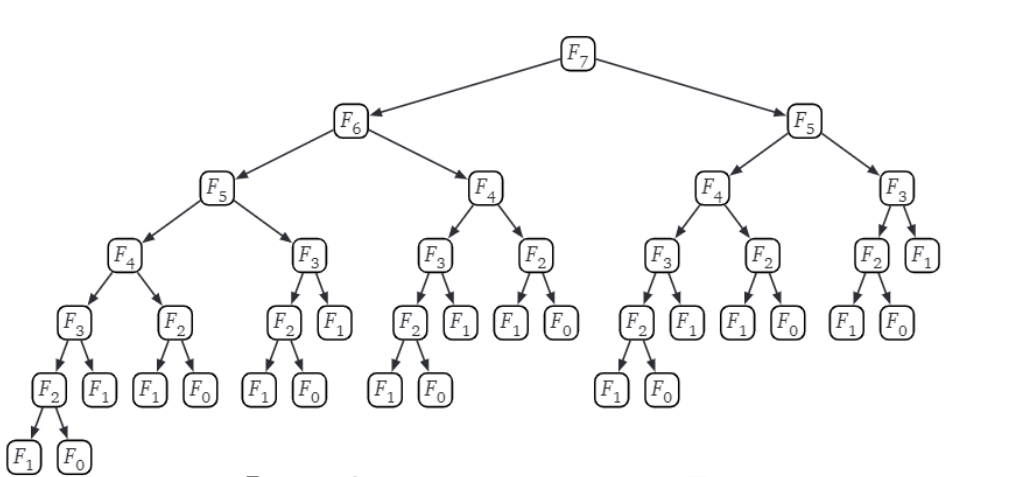
\includegraphics[scale=0.5]{figures/l9-1.png}
  \caption{\label{fig:fibtree} Recursive tree to compute $F_{7}$}
\end{figure}


\subsection{Memo(r)isation of recursion}

This method looks at the previous algorithm and asks whether it would be more efficient to store values on the first time they are computed so that they may be retrieved from a lookup table on subsequent recursions, for instance you can see that $F_{2}$ is recalculated in every sub-tree in Figure~\ref{fig:fibtree}, If we were to store it we could remove the need for this calculation to be repeated.

\begin{algorithm}
  \caption{MemoisationFibonacci}
  \uIf{$n=0$}{return 0}
  \uIf{$n=1$}{return 1}
  \If{$ F[n]$ is undefined}{
    $F[n] \leftarrow $ MemoisationFibonacci(n-1) + MemoisationFibonacci(n-2)
  }
\end{algorithm}

Using this algorithm we can trim or \textit{prune} the tree that needs to be generated.

\begin{figure}[ht]
  \centering
  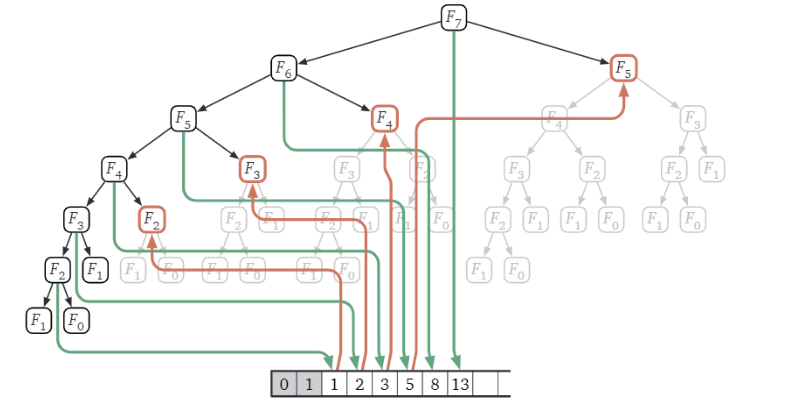
\includegraphics[scale=0.5]{figures/l9-2.png}
  \caption{\label{fig:memfib} Computing $F_{7}$ via memoisation}
\end{figure}

\subsection{Iterative approach}

At this point we are already maintaining an array, so why do we not fill it up iteratively? Recursion acts as a layer of abstraction, making our process closer to the formal (recursive) definition of the set. We can remove this and instead write our algorithm as:

\begin{algorithm}
  \caption{IterativeFibonacci(n)}
  $F[0] \leftarrow 0$

  $F[1] \leftarrow 1$

  \For{$i \leftarrow 2$ to $n$}{
    $F[i] \leftarrow F[i-1] + F[i-2]$
  }
\end{algorithm}

What is the running time of such an algorithm?

\begin{itemize}
  \item we store $n$ items in our array $F$
  \item Computing each new entry needs 2 lookups and one addition.

        Therefore, the total running time to compute $F_{n}$ is $O(n)$
\end{itemize}

\section{Interval Scheduling Problem}

\subsection{Without weights (lecture 8 recap)}

\begin{itemize}
  \item We are given a set of $n$ requests $R$ 

    $R = \{ \texttt{Req}(1), \texttt{Req}(2), \ldots, \texttt{Req}(i), \ldots, \texttt{Req}(n)\} $
  \item $\texttt{Req}(i)$ has a start time of $\texttt{Start} (i)$ and a finish time of $\texttt{Finish} (i)$
  \item There is a machine which can handle one request at a time
  \item Two requests \textbf{conflict} if they overlap
\end{itemize}

The interval scheduling problem asks:

\begin{problem}(Interval Scheduling)
 Select a set $C \subseteq R$ of requests such that $|C|$ is maximised and no two requests from $C$ conflict.
\end{problem}

\subsection{Weighted}

\begin{itemize}
  \item We are given a set of $n$ requests$ R$ 

    $R = \{ \texttt{Req}(1), \texttt{Req}(2), \ldots, \texttt{Req}(i), \ldots, \texttt{Req}(n)\} $
  \item $\texttt{Req}(i)$ has a start time of $\texttt{Start} (i)$ and a finish time of $\texttt{Finish} (i)$
        \item \textbf{Additionally, each request $\texttt{Req}(i)$ has a weight given by $\texttt{Weight}(i)$}
  \item There is a machine which can handle one request at a time
  \item Two requests \textbf{conflict} if they overlap
\end{itemize}

The weighted interval scheduling problem asks:

\begin{problem}(Weighted interval scheduling problem)
  Select a set $C \subseteq R$ of requests such that $\sum_{i\in C}\texttt{Weight} (i)$ is maximised and no two requests from $C$ conflict.
\end{problem}

I.e. maximise the weight of all chosen requests.

The algorithm seen for unweighted ISP does not hold. (Algorithm~)

\begin{algorithm}
  \caption{Select requests by increasing order to finish times}
  Let $R = \{ \texttt{Req}(1), \texttt{Req}(2), \ldots, \texttt{Req}(i), \ldots, \texttt{Req}(n)\} $ be the set of all requests

  Let $C$ denote the set of requests that we select, initialise it as $C = \emptyset $

  \While{$R \neq \emptyset$}{
    Find the request $\texttt{Req} (i) \in R$ which has the \textit{smallest} finish time.

    Add $\texttt{Req} (i)$ to $C$

    Delete from $R$ all requests that conflict with $\texttt{Req} (i)$
  }
\end{algorithm}
\textbf{Remember: } This is an example of a greedy algorithm. It does not take the newly added weights into account, therefore often finds a sub-optimal solution.

Instead to solve the weighted interval scheduling problem we:

\begin{algorithm}
  \caption{Weighted interval scheduling algorithm}
  Begin by ordering requests in increasing order of finishing time.

  $M[0] = 0$

  \For{each request $j\in 1..n$}{
    $M[j] = \max \{ \texttt{Weight}(j) + M[\texttt{Last} (j)], M[j-1]\} $
  }
\end{algorithm}

Where $\texttt{Last} (i)$ is given by:

\[
  Last(i) = \begin{cases}
    i &\text{the largest index $i$ s.t. $i$ is disjoint from $j$}\\
    0 &\text{if there is no request $i<j$ that is disjoint from $j$}
  \end{cases}
\]

and is the last compatible request with $i$.

In this algorithm, $M[j]$ stores the value of the set of requests of maximum weight which can be chosen for the sub-instance containing requests $\{ 1,2,\ldots,j \} $. Our goal is then to compute $M[n]$ from the entries $M[1],M[2],\ldots, M[n-1]$ (\textbf{Note} these have all been computed previously )

Our recurrence of $\max \{ \texttt{Weight} (j) + M[\texttt{Last} (j)], M[j-1] \} $ is basically deciding whether request $j$ is worth including in the final solution, if we had a higher total weight previously without $j$ then we can ignore it (keeping our previous value), but if not, our result is the weight of $j$ along with the result of the sub-instance concerned with the last compatible request with $j$ ($\texttt{Last}(j) $).

\subsubsection{Correctness}

We can prove the correctness of this algorithm by induction on $j$. Our base case will be $j=0$ and our inductive step essentially argues the correctness of our recurrence.

\subsubsection{Running time}

The running time of this algorithm can be broken down into:

\begin{itemize}
  \item Sorting the requests in increasing order of finishing time, this can be done in $O(n\log n)$ time.
  \item We can now find $\texttt{Last}(j) $ for $1 \leq j\leq n$ in $O(n)$ time.
  \item Filling $M[j]$ requires a comparison between two existing entries from $M$ along with an addition and a $\max$ operation. This can be done in $O(1)$ time.

        Therefore filling the entire array $M$ can be done in $O(n)$ time

\end{itemize}

\section{Bellman-Ford algorithm for finding shortest paths}

We have previously looked at Dijkstra's algorithm for finding shortest paths. However, this algorithm has one major flaw: it does not work when we have negative edge-lengths.

One might think a simple solution to this problem is to add a constant of the largest negative length to all edges in a graph. I.e. if the lowest edge value in a graph $G$ is $-2$, by adding $2$ to all edges there are no more negative edge lengths. This does not work in practise as it affects what paths are the shortest, preferring paths with fewer edges. (Change in path cost is equal to number of edges multiplied by the constant added).

An alternative algorithm that deals with this is the \textbf{Bellman-Ford} algorithm.

This algorithm assumes that there are no \textbf{negative cycles}. As this would imply that the optimal route is infinite in number of edges!

By assuming no negative cycles, we can say that for any two vertices $s$ and $t$, there is a shortest $s \rightarrow t$ path which has \textbf{at most} $n-1$ edges. We can show this to be correct:

\begin{itemize}
  \item Let $P$ be a shortest $s \rightarrow t$ path with the fewest number of edges.
  \item If a vertex $x$ repeats on $P$, then delete the $x\rightarrow x$ cycle from $P$
        \begin{itemize}
          \item Therefore the number of edges in $P$ decreases
          \item The length of $P$ cannot increase as there as no negative edges.
        \end{itemize}
\end{itemize}

\subsection{Defining our algorithm}

We can say, for each vertex $v \in V$ and each $0 \leq i \leq n-1$, let $\texttt{OPT} [i,v]$ denote the shortest $s \rightarrow v$ path having at most $i$ edges.

We can now set up our recurrence:

\begin{enumerate}
  \item If the shortest $s \rightarrow v$ path actually uses at most $i-1$ edges out of the original $i$ then the value is $\texttt{OPT} [i-1,v]$
  \item Otherwise, the last ($i^{th}$) edge has to be $(w,v)$ for some $w \in V$ as our shortest $s \rightarrow v$ path uses all $i$ edges.

        \begin{itemize}
          \item The cost of this path is $\texttt{OPT}[i-1,w] + \texttt{cost}(w,v)$
                \item We need to minimise this over all $w$ s.t. $(w,v)$ is an edge in $G$
        \end{itemize}
\end{enumerate}

We must take a minimum of these two choices:

\[
  \texttt{OPT}[i,v] = \min \left\{ \texttt{OPT}[i-1,v], \displaystyle\min_{w\in V}\left(\texttt{length}(w,v) + \texttt{OPT}[i-1,w]\right) \right\}
\]

We can now formulate our algorithm: (See Algorithm~\ref{alg:bf})

\begin{algorithm}\label{alg:bf}
  \caption{Shortest path from a vertex $s$ to all other vertices}
  We maintain a $n \times n$ table indexed by $0 \leq i \leq (n-1)$ and $v \in V$ where $\texttt{OPT} [i,v]$ stores the length of the shortest $s \rightarrow v$ path which uses at most $i$ edges.

  Define $\texttt{OPT} [0,s] = 0$ and $\texttt{OPT} [0,v] = \infty$ for each $v \in V, v\neq s$

  \For{$i = 1..n$}{
    \For{$v \in V$}{
      $\texttt{OPT} [i,v] = \min \left\{ \texttt{OPT} [i-1,v], \displaystyle\min_{w\in V}\left( \texttt{length}(w,v) + \texttt{OPT} [i-1,w] \right)\right\}$
    }
  }
  \Return $\texttt{OPT} [n-1,v]$ for each $v \in V$
\end{algorithm}

\subsubsection{Running time}

\begin{itemize}
  \item $\texttt{OPT} $ has $O(n^{2})$ entries
  \item Computing each entry needs to lookup (and compute )$O(n)$ entries.
        \begin{itemize}
          \item Computing $\texttt{OPT} [i,v]$ needs knowledge of $\texttt{OPT} [i-1,x], \forall x \in V$
          \item Needs to perform $O(n)$ $\min$ operations and $O(n)$ additions
        \end{itemize}
        \item Total running time $O(n^{3})$
\end{itemize}

\section{Subset Sum}

The subset sum problem is defined as:

\begin{problem}(Subset sum problem)
  Given $n$ items $\{ 1,2,\ldots,n \} $, where each item $i$ has a non-negative integral weight given by $\texttt{Weight}(i) $ and a  number $W$ as an \textbf{upper bound}.

  Find a set $S$ of items such that $\sum_{i\in S} \texttt{Weight} (i) $ is maximised subject to the constraint $\sum_{i\in S} \texttt{Weight} (i) \leq W $
\end{problem}

We can show that the greedy algorithm which always picks the item with the heaviest weight (while sum is at most $W$) fails.

We can show this by counterexample:

\begin{itemize}
  \item Item 1 has weight 15
  \item Item 2 has weight 25
  \item Item 3 has weight 15
\end{itemize}

Suppose we are given $W=30$.

Our greedy algorithm picks item 2 as it has the highest weight (while sum is at most $W$). But now it cannot pick either item 1 or 3 as then the sum would exceed $W$. However, we can see that the optimal solution is to pick items 1 and 3 to total 30.

In fact, we know that \textbf{no } greedy algorithm is known which can solve this problem optimally.

\subsection{A DP algorithm}

We can attempt to construct a dynamic algorithm to solve this problem:

Let $\texttt{OPT} [i]$ denote the max weight of choosing items from $\{ 1,2,\ldots, i \} $ such that sum of weights is maximised subject to being at most $W$.

Our final answer would therefore be stored in $\texttt{OPT} [n]$.

Similarly to Algorithm~\ref{alg:bf}, if an item $i$ is not chosen to be in our result set, $\texttt{OPT} [i] = \texttt{OPT} [i-i]$, i.e. we skip it and continue with our previous value.

However, if $i$ is chosen to be in the result set (at this point), then $\texttt{OPT} [i]$ contains $\texttt{Weight} (i)$ plus the optimal selection of items from $\{ 1,2,\ldots,i-1 \} $ with weight at most $W - \texttt{Weight} (i)$.

\textbf{Note} however, we do not store this value in $\texttt{OPT} [i-i]$, in this location we store the max weight of choosing items from $\{ 1,2,\ldots,i \} $ subject to $W$.

We therefore require a table to store this information.

For each $1 \leq i \leq n$ and $1 \leq X \leq W$, let $\texttt{OPT} [i,X]$ be the max weight of choosing items from $\{ 1,2,\ldots, i\} $ subject to weight totalling at most $X$.

\paragraph{Recurrence}

We can define our recurrence:

Let $\texttt{OPT} [i,X]$ be the max weight of choosing items from $\{ 1,2,\ldots,i \} $ subject to a max weight of $X$,

\begin{enumerate}
  \item If $i$ is \textbf{not} chosen,

        $\texttt{OPT} [i,X] = \texttt{OPT} [i-1,X]$ , this occurs if $\texttt{Weight} (i) > X$

  \item If $i$ is chosen,

        $\texttt{OPT} [i,X] = \texttt{Weight} (i) + \texttt{OPT} [i-1,X-\texttt{Weight}(i) ]$
\end{enumerate}


We can therefore construct the recurrence:

\[
  \texttt{OPT} [i,X] = \max \left\{ \texttt{OPT} [i-1,X] ; \texttt{Weight} (i) + \texttt{OPT} [i-1,X-\texttt{Weight}(i) ]\right\}
\]


This allows us to construct the following algorithm:

\begin{algorithm}
  \caption{Subset Sum($n,W$)}
  We maintain an $(n+1)\times (W+1)$ table indexed by $0 \leq 0 \leq n$ and $0 \leq X \leq W$ where $\texttt{OPT} [i,X]$ stores the max weight of choosing items from $\{ 1,2,\ldots,i \} $ subject to weight being at most $X$

  We initialise $\texttt{OPT} [0,Y]=0$ for each $0 \leq Y \leq W$

  \For{$i = 1,2,\ldots, W$}{
    \For{each $Z = 0,1,2,\ldots,W$}{
      $\texttt{OPT} [i,Z] = \max \{ \texttt{OPT} [i-1,Z]; \texttt{Weight}(i) + \texttt{OPT}[i-1,Z-\texttt{Weight}(i) ]   \} $
    }
  }

  \Return \texttt{OPT} [n,W]
\end{algorithm}

\subsubsection{Running time}

The table has $O(n\cdot W)$ entries. Filling a new entry in the table needs to look-up two existing entries from the table and perform one addition and one max operation. This can be done in constant time $O(1)$

Therefore, the time required to fill all entries is $O(n\cdot W)$.




\end{document}
